%%%%%%%%%%%%%%%%%%%%%%%%%%%%%%%%%%%%%%%%%
% University/School Laboratory Report
% LaTeX Template
% Version 3.1 (25/3/14)
%
% This template has been downloaded from:
% http://www.LaTeXTemplates.com
%
% Original author:
% Linux and Unix Users Group at Virginia Tech Wiki 
% (https://vtluug.org/wiki/Example_LaTeX_chem_lab_report)
%
% License:
% CC BY-NC-SA 3.0 (http://creativecommons.org/licenses/by-nc-sa/3.0/)
%
%%%%%%%%%%%%%%%%%%%%%%%%%%%%%%%%%%%%%%%%%

%----------------------------------------------------------------------------------------
%	PACKAGES AND DOCUMENT CONFIGURATIONS
%----------------------------------------------------------------------------------------

\documentclass{article}

\usepackage[version=3]{mhchem} % Package for chemical equation typesetting
\usepackage{siunitx} % Provides the \SI{}{} and \si{} command for typesetting SI units
\usepackage{graphicx, xcolor} % Required for the inclusion of images
\usepackage{natbib} % Required to change bibliography style to APA
\usepackage{amsmath} % Required for some math elements 
\usepackage{svg} % .svg support
\usepackage[nolist]{acronym}
\usepackage{minted}
\definecolor{bg}{rgb}{0.95,0.95,0.95}

\graphicspath{{img/}}

\setlength\parindent{0pt} % Removes all indentation from paragraphs

\renewcommand{\labelenumi}{\alph{enumi}.} % Make numbering in the enumerate environment by letter rather than number (e.g. section 6)

%\usepackage{times} % Uncomment to use the Times New Roman font

%----------------------------------------------------------------------------------------
%	DOCUMENT INFORMATION
%----------------------------------------------------------------------------------------

\title{Projekt: Mobilfunk und Singalverabreitung} % Title

\author{Lukas Becker, Tobias Frahm} % Author name

\date{\today} % Date for the report

\begin{document}

\maketitle % Insert the title, author and date

\begin{center}
\begin{tabular}{l r}
Date Performed: & \today \\ % Date the experiment was performed
Partners: & Lukas Becker, Tobias Frahm \\ % Partner names
Instructor: & Prof. Dr. Sauvergerd \\% Instructor/supervisor
University: & University of Applied Science 
\end{tabular}
\end{center}

\begin{acronym}
    \acro{CPFSK}{Continus Phase Frequency Shift Keying}
\end{acronym}

% If you wish to include an abstract, uncomment the lines below
% \begin{abstract}
% Abstract text
% \end{abstract}

%----------------------------------------------------------------------------------------
%	SECTION 1
%----------------------------------------------------------------------------------------

\section{Projektbeschreibung und Ziel des Projektes}

In diesem Projekt wird eine \ac{CPFSK} Demodulation von Wetterdaten 
(Seewetterbericht des  Senders  Pinneberg  auf  Kurzwelle)  in  Echtzeit  durchgeführt. 
Diese  \ac{CPFSK} Demodulation  wird  in  Form  eines  \textit{Software  Radios}  auf  einem  
Digitalen Signalprozessor (DSP) implementiert. 

Die \ac{CPFSK}-kodierten Wetterdaten werden mit einer Draht-Antenne im Frequenzebereich
$10.1Mhz$ bis $11.1MHz$ empfangen und verstärkt. Bei dem so empfangenem Signal handelt es sich um 
\ac{CPFSK}-Modulierte Seewetterdaten. Ziel das Projektes ist es, zunächst in Matlab ein Modell zu erstellen, welches
in der Lage ist, die \ac{CPFSK} modulierten Seewetterdaten zu decodieren und diese auszugeben. 
Für das Matlab Modell wird hierfür zunächst ein \ac{CPFSK}-Signal in Matlab erzeugt um die ersten 
Schritte durchzuführen. Später in der Simulation kann hier auf ein Zeitbegrenztes Signal 
als Grundlage für das Matlab Modell genutzt zurückgegriffen werden. 
Sobald das Matlab Modell steht, wird die Simulation in C-Code überführt und anschließend 
auf einem DSP implementiert.

\section{Simulation: Matlab}
In dem folgenden Kapitel wird zunächst ein Rechteckimpuls auf eine Trägerfrequenze mithilfe der \ac{CPFSK} moduliert.

\subsection{CPFSK Modulation}
Die \ac{CPFSK} Modulation ist eine Methode um digitale Signale mithilfe einer Trägerfrequenze analog zu Übertragen.
Bei der \ac{CPFSK} Modulation handelt es sich um eine Frequenzmodulation ohne Sprünge im Phasenübergang. In Abb.~\ref{fsk}
ist im oberen Bereich das binäre Signale, im mittleren Bild die Trägerfrequenze und unten das binäre Signal auf die Trägerfrequenze
moduliert zu sehen. Der Phasenübergäng ohne Sprung ist notwendig, da Sprünge ein theoretisch unendliches breites Band benötigen
somit die Nachbarkanäle stören würde.
\begin{figure}[!h]
    \centering
    \def\svgscale{0.3}
    \def\svgwidth{\columnwidth}
    \input{img/fsk.pdf_tex}
    \caption{Beispielhaftes \ac{CPFSK} moduliertes Trägersignal einer binären 
    Information. Die Phasenübergänge sind ohne Sprung. Quelle:~\cite{wiki:fsk}}
    \label{fsk}
\end{figure}
\subsection{Rechteckimpuls $d(i)$}\label{sec:rechteck}
Mit Angabe der Symboldauer $T = 20ms$ lässt sich auf die minimale Abtastfrequenz nach Nyquist-Shannon schließen.
Die minimale Abtastfrequenz $f_A$ muss mehr als doppelt so groß wie die höhste abzutastende Frequenz sein.


Aus
\begin{center}
 $
f_A > 2*f_{max}
$
\end{center}

mit 
\begin{center} $f_{max} = \frac{1}{T_{max}} ; T_{max} = T = 20ms$  \end{center}

ergibt sich

\begin{center}
$
f_A > 2*\frac{1}{T}
$
\end{center}

Eingesetzt:
\begin{center}
$f_A > 2*\frac{1}{20ms}$
\end{center}
\begin{center}
$f_A > 100Hz$   
\end{center}
\begin{figure}[!h]
    \centering
    \def\svgscale{0.3}
    \def\svgwidth{\columnwidth}
    \input{img/rechteck.pdf_tex}
    \caption{Recheckimpuls zur \ac{CPFSK} Simulation in Matlab}
\end{figure}

\subsection{Anfangsphase $\phi(iT)$}

Gegeben ist die ein Integrator (IIR Filter 1.Ordnung) mit der Übertragnungsfunktion:
$$
H_I(z)=\frac{z^{-1}}{1-z^{-1}}
$$
Dieser kann hier anstelle der Summenbildung der komplexen Einhüllenden eingesetzt werden, 
da die Integration einer Aufsummierung diskreter Flächenelemte unter der Kurve entspricht.

\begin{figure}[!h]
    \centering
    \def\svgscale{0.3}
    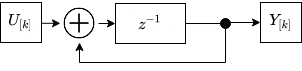
\includegraphics{img/sig_IIR.png}
    \caption{Signalflussdiagramm des Integrators 1.Ordnung}
\end{figure}

\subsection{CPFSK Signal}
Das in Abschnitt~\ref{sec:rechteck} generierte Reckecksignal wird nun CPFSK Modeliert.
Dafür wir die Formel aus Worksheet 1 verwendet:

$$CPFSK_{sig} = amp \cdot  sin(2  pi \cdot f_T \cdot n \cdot T_A + 2 pi \cdot \varDelta{F} \cdot \frac{\phi (iT)}{f_A} + \varphi{0}) $$

Zur bestimmung des Spektrums des Signals, wird in Matlab FFT verwendet.
\begin{figure}[!h]
    \centering
    \def\svgscale{0.3}
    \def\svgwidth{\columnwidth}
    \input{img/spektrum.pdf_tex}
    \caption{Betragspektrum des CPFSK-Modulierten Rechteckimpulses.}
\end{figure}
Bei einem $\varDelta(F) = 225Hz$ wird hier eine Bandbreite von ca. $B > 450Hz = 2\cdot \varDelta(F) $ erwartet.

Zur Bandbreitenbestimmung wird das Parsevalsche Theorem genutz, die Bandbreite des CPFSK Signals ist derjenige Bereich,
in den 99\% der Signalenergie von $0...\frac{f_A}{2}$ Fallen.

$$
\sum_{n = 0}^{N - 1}\left\lvert x(n)^2\right\rvert =  \frac{1}{N} \sum_{k = 1}^{N-1}  \left\lvert X(k)^2\right\rvert 
$$

\begin{minted}{matlab}
% Die Bandbreite wird durch den Breich beschrieben, in den 99% der
% Signalenergie fallen.

total_power = 0;
current_power = 0;
idx = 0;
idx_max = round(length(spectrum_sig)/2);
idx_start = idx_max/2; % fA/4

for i = 1:length(spectrum_sig)/2 - 1
    total_power = total_power + abs(spectrum_sig(i))^2 / length(spectrum_sig);
end

N = length(spectrum_sig);

while current_power/total_power < 0.99
    current_power = current_power + abs(spectrum_sig(idx_start - idx))^2 / N;
    current_power = current_power + abs(spectrum_sig(idx_start + idx))^2 / N;
    idx = idx + 1;
end

fprintf("Bandbreite: %dHz\n", ((idx_start + idx) - (idx_start - idx)))
\end{minted}


---------------------------------------------------------------------------
%	BIBLIOGRAPHY
%----------------------------------------------------------------------------------------

\bibliographystyle{apalike}
\bibliography{lib}

%----------------------------------------------------------------------------------------


\end{document}